\section{Background}
Poker software has been developed before by multiple companies, but these
are all mostly commercial, closed source software, with no discussion of the
algorithms and design decisions that went into them. This project will go
into depth on some of the issues that are faced when converting the game of
poker from the table to the computer.

\subsection{How To Play Poker}
Each player is dealt two cards, and the player to the left of the dealer must
pay a small bet, called the small blind, with the player to his left paying 
double this bet, the big blind. Play then proceeds clockwise from the next
player. Each player has the option to fold, check, call, raise, or go all in,
depending upon the circumstances. Folding forfeits any stake in the round, and
removes you from play. Checking means you wish not to bet, and is only
available if there is no current bet which needs matching. Calling means to
match the current bet, and raising means to raise the current bet to a higher
value. Going all in means to bet all your chips, and sometimes is mandatory to
remain in the pot, if you have less chips than the current bet. This can cause
multiple side pots to occur. Each player has an amount of chips at the 
beginning of the game which they bet with, these may be backed by real money as
is the case in casinos and most online poker software. Once all players have
matched the current bet or folded, three table cards are revealed, called
the flop. These are common to all players hands, and may be used along with
the players two hidden cards to form the best 5 card hand. A further two table
cards will be revealed as play continues, unless all players but one fold,
leaving the winner to keep any bet chips. Again, players may bet if they wish.
Providing there are still players in play, the fourth card will be revealed, 
called the turn. The same process occurs again, then the fifth card will be
revealed, the river. Once this betting round has ended, any players still
in play reveal their cards, and the winner is the player who has the best
five card hand. These can vary from simple pairs, to higher valued hands such
as a straight, which is five cards in a row, such a 5, 6, 7, 8, 9. The winner
receives all the chips in the middle of the table gained from other players
bets, and a new round begins, with the dealer moving to the next player on the
left.

\subsection{Randomness and Shuffling}
In the game of poker, the house does not wager against players. In each
poker hand, a player always wins, unlike other popular casino games, such as 
blackjack or roulette. Instead the usual method for online poker companies and
indeed poker tables in real life to make money is the rake. The rake is the 
commission fee that a casino takes from players in some method, as their way 
of generating revenue.

The implementation of the rake varies between casinos and online poker
software. Some common ones are in the below table.

\begin{center}
    \begin{tabular}{l l}
    \toprule
    Mechanism           & Description                                               \\
    \midrule
    Pot Rake            & Percentage taken from the pot, per hand or betting round  \\ \addlinespace
    Dead Drop           & Fee paid by the player with the dealer button each hand   \\ \addlinespace
    Timed Rake          & Set fee collected every set interval of time              \\ \addlinespace
    Fixed Fee           & Fixed fee per hand                                        \\ \addlinespace
    Tournament Fee      & Entry fee to participate in poker tournaments             \\ \addlinespace
    Subscription Fees   & Players are charged a subscription fee to play            \\
    \bottomrule
    \end{tabular}
\end{center}

Finally, some games are rake free, instead generating revenue by driving
traffic to more profitable businesses. The software developed that this paper
is discussing is also rake free, due to being only for academic purposes.

However, despite companies being able to generate revenue in these ways, the
implementation of random number generation in poker software is a topic of
some interest. Possible issues include rogue employees writing malicious
code to give them or people connected to them beneficial cards, faulty code
allowing the random number generation to be exploited, and other schemes, such
as giving newer players or failing players better cards, to encourage them to 
continue using the companies platform, and generating revenue through rakes.

For these reasons, random number generation has been analysed and multiple
different shuffling algorithms or card picking algorithms have been
developed and contrasted for possible weaknesses. Two obvious approaches to 
selecting cards are:

\begin{itemize}
    \item Storing an array of all the cards and indexing this array in some way to take a card
    \item Shuffling an array in some way and taking the top item
\end{itemize}

\newpage

It was hypothesised that the random number implementation and card picking
algorithms could effect the cards generated, and potentially lead to a more
predictable, non random game. For this reason, multiple algorithms and
different sources of randomness has been developed and tested, along with two
complementary programs to test them. Firstly, a GUI which can be launched
when the `--chooseshuffle' argument is given to the server, allows the card
picking algorithm and random source to be altered mid game.

This program simply allows the user to change the shuffle and random source
by picking from a list. Once this item is changed, internally a variable is
assigned to the new chosen shuffle and random source, and upon the round
being completed, the method for drawing cards is updated with the new user
selected function. This prevents the method being changed mid round, which
has a high potentially to cause bugs, due to the deck state having to be
maintained. Upon subsequent rounds, the new chosen functions will be used
to draw cards.

\begin{figure}[H]
    \centering
    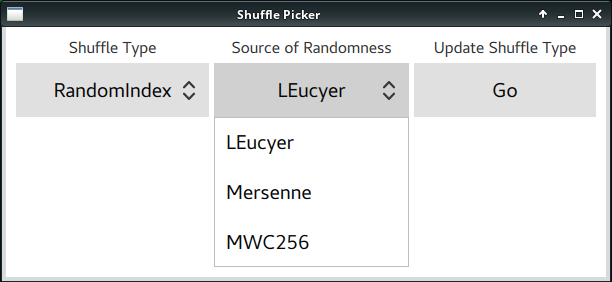
\includegraphics[width=0.8\linewidth]{../images/shufflepicker.png}
    \caption{The Shuffle Picker Window}%
    \label{fig:shufflepicker}
\end{figure}

Another program provides a similar interface but instead allows multiple hands 
to be drawn and the number of times each card was drawn displayed in a graph. 
This allows us to easily see the effect of the different algorithms on the 
uniformness of the card distribution. Each iteration draws 17 cards from
a new deck. This number is chosen because in this implementation of the game,
the maximum number of players is 6, and there are 5 cards displayed on the
table. Hence, with 2 cards each, $2 * 6 + 5 = 17$. As each card is drawn,
it is added to a card dictionary. If the card already exists, the number seen
of this card is incremented. If not, the card is inserted, with an initial
value of 1. 

\begin{figure}[H]
    \centering
    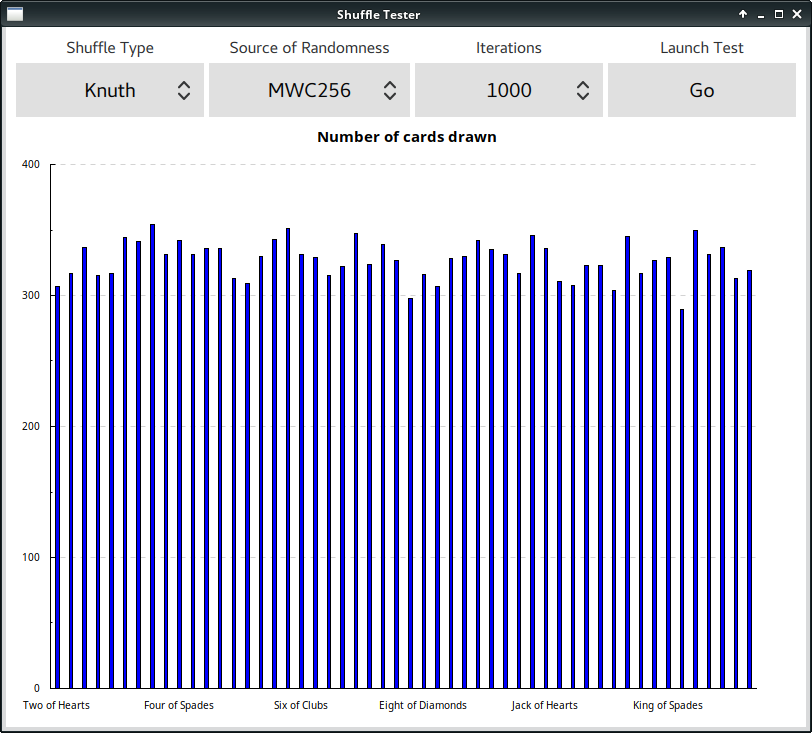
\includegraphics[width=0.8\linewidth]{../images/shuffletester.png}
    \caption{The Shuffle Tester Program}%
    \label{fig:shuffletester}
\end{figure}

Algorithm~\ref{code:shuffletester} describes this programs high
level execution.

\vspace{0.3cm}

\begin{algorithm}[H]
    \nlset{STEP 1} launch GUI\;
    \While{close button not pressed}{
        \If{go button pressed}{
            \nlset{STEP 2} $iterations \leftarrow \text{selected number of iterations}$\;
            $drawFunction \leftarrow \text{selected card draw function}$\;
            $randomSource \leftarrow \text{selected source of randomness}$\;
            $cardMapping \leftarrow []$\;
            \nlset{STEP 3} \For{$i \leftarrow 0$ \KwTo{} $iterations$}{
                $deck \leftarrow \text{new deck}$\;
                $cards \leftarrow []$\;
                \For{$j \leftarrow 0$ \KwTo{} $17$}{
                    \nlset{STEP 4} $card \leftarrow drawCard(drawFunction, randomSource, deck)$\;
                    \If{$card$ \text{is member of} $cardMapping$}{
                        cardMapping[card]++\;
                    }
                    \Else{
                        insert ($cardMapping$, $card$, 1)\;
                    }
                }
            }
            \nlset{STEP 5} $barChart \leftarrow []$\;
            \nlset{STEP 6} \For{$i \leftarrow 0$ \KwTo{} length ($cardMapping$)}{
                createBar ($barChart$, $cardMapping[i]$)\;
            }
            \nlset{STEP 7} display ($barChart$)\;
        }
    }
\caption{The shuffle tester algorithm}%
\label{code:shuffletester}
\end{algorithm}

\vspace{0.3cm}

The three sources of randomness used are:

\begin{itemize}
    \item Portable Combined Generator of L'Eucyer \parencite{leucyer1988}
    \item Faster Mersenne Twister \parencite{matsumoto1998,saito2008}
    \item Multiply With Carry 256 \parencite{marsaglia2003}
\end{itemize}

\begin{center}
    \begin{tabular}{l l l}
    \toprule
    Random Source           & Bit Size  & Cycle Length  \\
    \midrule
    L'Eucyer                & 32        & $ \displaystyle \frac{(2147483563-1)(2147483399-1)}{2}$   \\ \addlinespace
    Fast Mersenne Twister   & 128       & $ \displaystyle {2}^{19927}-1$                            \\ \addlinespace
    Multiply With Carry 256  & 32        & $ \displaystyle {2}^{8222}$                               \\
    \bottomrule
    \end{tabular}
\end{center}

These cycle lengths are sufficiently long that it would be very difficult
for an attacker to use the knowledge of the period length to their advantage,
as even the algorithm with the lowest cycle (L'Eucyer's), allows for
approximately $1.35e17$ hands to be dealt before the generator cycle ends.

The bit size is not an issue in the RandomIndex and KnuthShuffle
implementation, as they only require random numbers to be equally distributed
between 0 and 51. However, RandomSort generates one random number for each
card, then sorts the card list based on the number generated. Therefore, if
the same number is generated more than once, the shuffle will be non random.
We can compute the probability of the same number being picked more than once
using equation~\ref{eq:probSameNumSimple}.

\begin{equation} \label{eq:probSameNumSimple}
\begin{split}
& k = 2^\text{bit size}\\
& p = 1 - \frac{k!}{{k^{52}}(k - 52)!}
\end{split}
\end{equation}

Factorials of the large numbers we are using are numerically complex to
calculate, so a simplification is shown in equation~\ref{eq:probSameNumFast}.

\begin{equation} \label{eq:probSameNumFast}
\begin{split}
& k = 2^\text{bit size}\\
& p = 1 - \frac{\displaystyle\prod_{i=0}^{51} k - i}{k^{52}}
\end{split}
\end{equation}\\

If we have a 32 bit number, $p = 3.08\num{e-7}$.\\
For a 128 bit number, $p = 3.89\num{e-36}$.\\

Therefore, the chance of the same number being picked more than once is small,
and so the shuffle has a high probability to be uniform.

Whilst testing the shuffles with the shuffle tester, it was discovered that
the Knuth shuffle with the Mersenne twister algorithm would deal cards in a
non uniform manner. As we can see in~\ref{fig:faultymersenne}, the first 17
cards in the deck were approximately 5\% less likely to be drawn.

\begin{figure}[H]
    \centering
    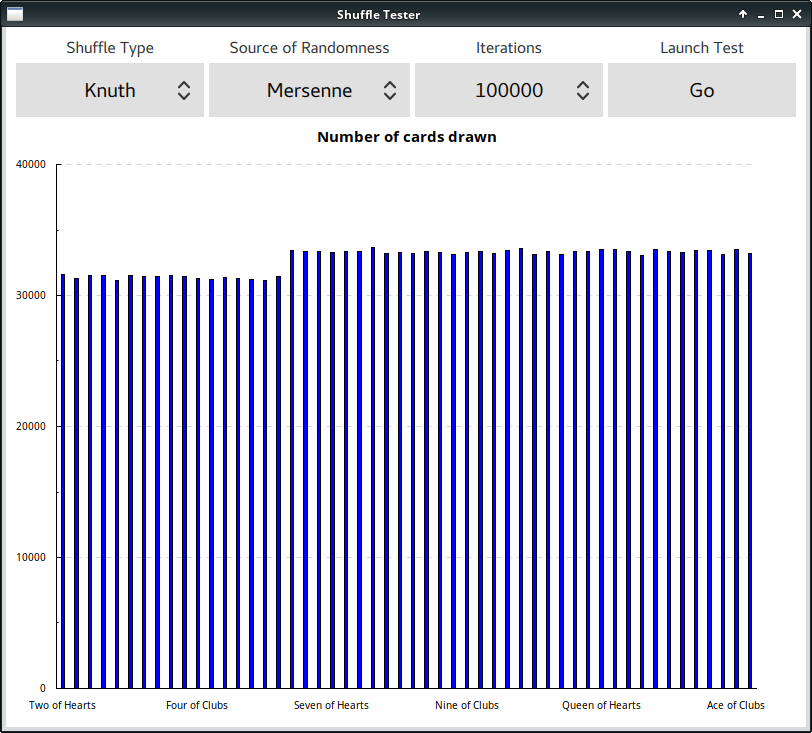
\includegraphics[width=0.8\linewidth]{../images/faultymersenne.png}
    \caption{The Non Uniform Mersenne Distribution}%
    \label{fig:faultymersenne}
\end{figure}

This was due to the random library having no function allowing random numbers
within a range to be generated, and instead a na\"{\i}ve implementation was
used, as in Algorithm~\ref{code:rngBadCapping}. In this version of
getRandomNumber, no bounds are given, and the function simply returns a
random number in the range of an integer.

\vspace{0.3cm}

\begin{algorithm}[H]
    \SetKwInOut{Input}{input}\SetKwInOut{Output}{output}
    \Input{An integer $maxValue$}
    \Output{A random number of maximum $maxValue$}
    \BlankLine{}
    \nlset{STEP 1} $x \leftarrow getRandomNumber$\;
    \nlset{STEP 2} return $x$ \% $maxValue$\;
\caption{Initial random number capping implementation}%
\label{code:rngBadCapping}
\end{algorithm}

\vspace{0.3cm}

Due to the the values not begin distributed evenly, this resulted in the
above non uniform distribution. This was solved by using an algorithm in which
all the possible values of the random number generator are divided into equal
sized intervals, each representing one of the desired values. For example
if the maximum number the random number generate can create is 11, and the
desired values are a range from 0 to 5, \{0,1\} would be assigned to 0, \{2,3\}
to 1, and so on. This new version can be seen in
Algorithm~\ref{code:rngGoodCapping} \parencite{website:reich2011}.

\vspace{0.3cm}

\begin{algorithm}[H]
    \SetKwInOut{Input}{input}\SetKwInOut{Output}{output}
    \Input{An integer $maxValue$}
    \Output{A random number of maximum $maxValue$}
    \BlankLine{}
    \nlset{STEP 1} $range \leftarrow 1 + maxValue$\;
    \nlset{STEP 2} $buckets \leftarrow {2}^{32}\; / \;range$\;
    \nlset{STEP 3} $limit \leftarrow buckets \times range$\;
    \nlset{STEP 4} $x \leftarrow 0$\;

    \nlset{STEP 5} \While{$x$ $<$ $limit$}{
        $x \leftarrow getRandomNumber$\;
    }

    \nlset{STEP 6} return $x$ / $buckets$\;
\caption{Revised random number capping implementation}%
\label{code:rngGoodCapping}
\end{algorithm}

\vspace{0.3cm}

To an extent this demonstrates how easy it would for poker software to have
biased distributions if rigorous testing procedures were not in place.

After implementing the above shuffle tester, and comparing the results,
it was concluded that all shuffles and sources of randomness appear at face
level to be sufficiently random, and not effected by the implementation chosen.
However, as early mentioned, it is very simple for an implementation to be
incorrectly developed, causing non random cards to appear.

A simple way for a malicious actor to generate cards which appear to be random
but actually benefit or hinder a player is to generate cards in a random
way, as in one of the above algorithms, then inspect the generated cards,
and distribute them to players in a specific way to cause the desired effect.
For example, if there were 3 players, and the generated cards were
[Ace, Ace, Seven, Seven, Two, Two], both the aces could be distributed to
the player who has the least chips, whilst the other two players both receive
a seven and two, the statistically worst hand in Texas Hold-Em Poker.

Using this method of rewarding the players with less chips, whilst the overall 
hands and cards generated will be uniform, the cards dealt to each player 
will not be. This could still be measured, but is harder to do so. If the
method is repeatedly applied, in that a player will gain chips by being dealt 
favourable hands and lose chips when dealt bad hands, the player would have 
a cycle of good to bad cards dealt to him as his chips decrease and increase, 
and so might be difficult to detect over long periods, as the highs and lows 
would cancel out.

However, this would be possible to detect if a player is particularly good, or
particularly bad. If they are particularly good, and play their bad hands well
to minimise their chip loss, they will over long periods have a non uniform
card distribution due to constantly having more chips than the average player.

Again, this can be mitigated by dealing uniformly distributed cards to all
players, but instead manipulating the table cards, so flops which benefit
the players with less chips' hands. In this way, a good player still receives
the amount of AA hands as a poorer player, but upon having this AA hand will
find that other players achieve three of a kinds, two pairs, flushes etc
with their lower ranked hands.

Software with rigged gameplay has been observed in the wild too. In 2011 
`BLR Technologies' was discovered to have been utilising rigged odds, with an 
observed win rate of $24.70\%$ compared to an expected win rate of $49.29\%$,
after having played 328 rounds. The chance of this occurring is 1 in 
146,107,962. \parencite{website:shackleford2011} After these allegations, 
the companies software was dropped by a casino software aggregator, `5Dimes'.

In conclusion, whilst we can demonstrate random number generation algorithms
to be hard or impossible to manipulate by the end user, the creator can do so
in harder and harder to detect ways to the casino's benefit. It is for this
reason that casinos must be transparent about their algorithms and allow
for rigorous investigation by standards agencies.
